\documentclass[10pt, letter]{article}
\newcommand{\doctitle}{%
Solving Raven's Test of Intelligence using Visual Representation}
\newcommand{\bigO}{\ensuremath{\mathcal{O}}}
\newcommand{\tab}{\hspace*{12em}}
\usepackage{graphicx}
\usepackage{float}
\usepackage{listings}
\usepackage{comment}
\usepackage{fancyvrb}
\usepackage{booktabs}
\usepackage[usenames,dvipsnames]{color}
\usepackage[center]{caption}
\usepackage{algorithm}
\usepackage{algpseudocode}
\usepackage[margin=1in]{geometry}
\usepackage[usenames,dvipsnames]{color}
\usepackage{hyperref}
\hypersetup{
  colorlinks,
  citecolor=Violet,
  linkcolor=Black,
  urlcolor=Blue}
\begin{document}
\title{\textbf{\doctitle}\\
\textsc{Project \#4}
}
  \author {Arvind Krishnaa Jagannathan \\ GT ID: 902891874}
   \date{November 25, 2012}
\maketitle

\section{Introduction}
\subsection*{Raven's Test for Intelligence}
Raven's test for intelligence usually involves questions of the type A:B::C:x, where A,B,C are usually images which have some implicit relations. x is an unknown image, which needs to be selected from a set of given options, based on which of the choices best ``fit'' into the inferred relation. The goal of this project is to be able to correctly solve 10 (+2) such problems, from their visual representations, both by a purely ``visual'' approach as well as deriving propositions out of those representations. 

In assignment 3, I have used the purely ``visual'' approach and thus the new approach in this assignment is the ``propositional'' method. The propositions extracted from the images are different from the handcoded ones I used for project 2. I have detailed the structure of the propositions in the Design section.

\subsection*{Representation of problems for the Raven's Test}

Two methods are applied to solve each problem in the Raven's test, purely visual and by extracting propositions. However for both these methods, the input visual representation is the same, which is the GIF file of the given problem split up into several images, each representing one frame of the problem statement. The split up files are categorized into two: (a) Reference (b) Solution. The image files for each problem is placed by convention as depicted in Figure \ref{fig2}.

\begin{figure}[h!]
  \centering
    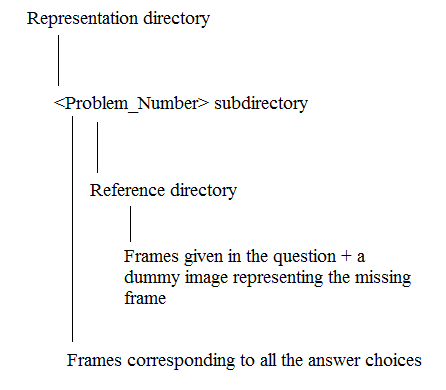
\includegraphics[scale = 0.6]{Images/Fig2}
    \caption{Structure of the visual representation directory}
  \label{fig2}
\end{figure}

A dummy image is placed in the ``Reference'' folder, so that the dimensions of the problem can be simply found by finding the square root of the number of items in the Reference folder. This dummy image is the problem GIF file.

\begin{figure}[h!]
  \centering
    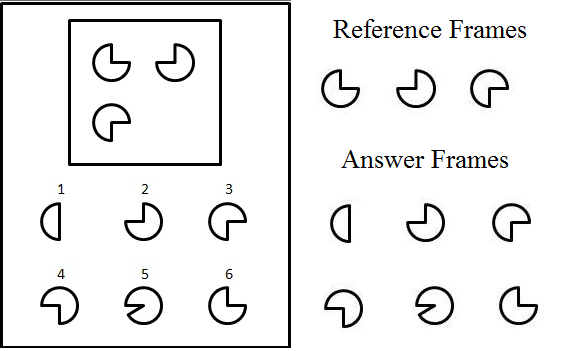
\includegraphics[scale = 0.5]{Images/Fig1}
    \caption{Visual Representation of a problem used in this project}
  \label{fig1}
\end{figure}

\section{Design of the Problem Solver}
\subsection*{Some Key Assumptions}
The program was designed to solve problems of analogical reasoning in a way I would typically solve them. Although I was unable to capture every step in my reasoning process,  I have assumed that some particular parts of my reasoning approach would be universal and the program has incorporated that. 
	\subsubsection*{Assumption \#1}
Frames are usually inspected from left to right in a particular row. I assume that the first frame would act as a sort of ``base" frame and any differences or transitions of subsequent frames can be described with respect to the properties of this frame.
	\subsubsection*{Assumption \#2}
In problems of dimensions 3x3, I have assumed that if we find an answer such transitions in that row correspond to those in rows 1 and 2 of the reference matrix, then that is the answer. In other words, I have assumed that if row correspondence match, then column correspondence would ``fall-in-place''.
	\subsubsection*{Assumption \#3: Image correctness}
The visual analogy solver works on a pixel-by-pixel match in order to find the relevant structural transition from one frame to another. In most real world image formats, random pixels may appear out of place in the image due to the compression algorithm used (in my case JPG). For the best results, it is assumed that each of the visual representations for a given problem is ``noise free''. To achieve this, each image has been manually processed to remove as much of noise as possible.
	\subsubsection*{Assumption \#4: Image orientation and size}
This assumption is also a result of the visual analogy solver working on the level of pixels. Each of the individual frames are expected to be of exactly the same dimensions. In this project each frame has a dimension of 79x79 pixels. Although it is not necessary for the dimensions to be that of a square, it is vital that the number of pixels to compare are the same (hence the restriction on the dimensions). It is also assumed that the orientation of the frame is reproduced exactly as it is the problem, suited to fit the dimensions of the visual representation. This means that the amount of whitespace around the shapes, the alignment of each shape and the relative distance between the shapes of each frame from the original problem GIF image need to be preserved in the 79x79 representation. Figure \ref{fig3} represents the correct reproduction of the problem frame, as well as a few ``incorrect'' ones. The rectangular border around each orientation is just to give an idea of the position of the frame with respect to the dimensions of the representation; the actual representation does not contain this.
\begin{figure}[h!]
  \centering
    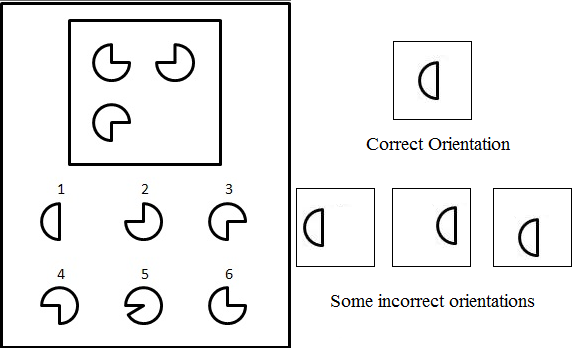
\includegraphics[scale = 0.5]{Images/Fig3}
    \caption{Preserving the relative characteristics of each frame}
  \label{fig3}
\end{figure}
	\subsubsection*{Assumption \#5: What is an exact match?}
Although two images seem to be matching exactly from a human point-of-view, when a pixel-by-pixel comparison is done, some finite difference may exist. Thus it is necessary to define certain thresholds within which if the pixel difference between two images fall, then they are considered to be matching. The following thresholds are established, experimentally, for various matching scenarios:
	\begin{enumerate}
		\item If image1 needs to checked for an exact match with image2 (i.e check if image1 == image2), then the comparison difference threshold is 200.
		\item If it needs to be checked if \\
		\centerline{Shapes(image1) - Shapes(image2) == Shapes(image3) - Shapes(image4)}\\
		then the threshold is 650.
		\item If it needs to be checked if \\
		\centerline{Shapes(image1) / Shapes(image2) == Shapes(image3) / Shapes(image4)}\\
		then the threshold is 50.
	\end{enumerate}
All these values are purely experimental (outlined in the \emph{Introspection} section) and may or may not be accurate since the number of problems used to arrive at these empirical values are very few.\\
\textbf{Note}: The pixel difference between two images is obtained as a correlation measure of the RGB matrix. It is mentioned in more detail in the subsequent section.
\subsubsection*{Assumption \#6}
In problems of visual reasoning people often find the ``macro'' differences between each frame, such as a missing shape or an addition of a new shape, before drilling down to ``micro'' differences such as the change in orientation, its color and so on. My program may not exhaustively capture all these differences, but it captures the ``macro'' differences and then uses that to filter the answer choices to a subset of the original choices, for which the ``micro'' differences are captured.

\subsection*{Algorithm}
There are two algorithms being employed in this assignment. One is the the visual analogy solver which is implemented verbatim from the previous assignment, and the other is using the visual solver to derive simple propositions which will then be utilized to obtain the solution for each of the problems. 

\subsubsection*{Purely Visual Solver}
The visual solver uses the idea that each frame in a given row or column of the problem matrix are connected by similitude transformations \cite{paper}. The visual solver attempts to find this transformation from the frames of the ``source'', which is the reference frames of each problem and then apply this transformation to ``incomplete'' row of the problem and obtain an estimate of what the right answer would be. Then each of the answer choices are compared with this estimated answer, and the one which is ``closest'' to this estimate is selected as the correct answer.

\subsubsection*{Extracting propositions out of the visual representations}
In the propositional solver, a ``simple'' representation is created for each of the answer choices. A base representation is created for each of the frames in the reference matrix as well as the incomplete matrix. Then each of the answer choices is picked one-by-one and placed along with the representations of the frames in the incomplete matrix. The representation so constructed is then compared with the representations of the reference frames. Each of the answer choices are assigned a score based on the level of correlation between the reference matrix and the newly constructed matrix. The answer choice which gives the highest correlation score is chosen as the right answer.

\subsection*{Visual Analogy Solver}
The visual analogy solver is dependent on the dimensions of the problem, i.e., the method of deriving the estimate will differ between a 2x2 problem and a 3x3 problem. Before I detail the steps for the 2x2 and 3x3 problems, I will outline the convention used for representing each of the frames in a given problem. For a 2x2 problem, the frames in the first row are Frame1-1, Frame1-2 and the frame in the second row (the incomplete matrix) is Frame2-1. The answer frames are numbered 1, 2, ..., $n$. For a 3x3 problem, the frames in the first row are Frame1-1, Frame1-2, Frame1-3 and the frames in the second row are Frame2-1, Frame2-2, Frame2-3. The frames in the final row are Frame3-1, Frame3-2 and the answer frames are numbered similar to a 2x2 problem. Figures \ref{fig4} and \ref{fig5} depict these conventions.

\begin{figure}[h!]
  \centering
    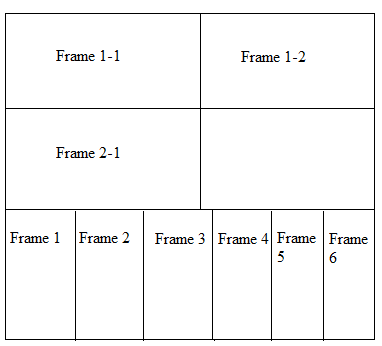
\includegraphics[scale = 0.4]{Images/Fig4}
    \caption{Convention for representing the frames in a 2x2 problem}
  \label{fig4}
\end{figure}

\begin{figure}[h!]
  \centering
    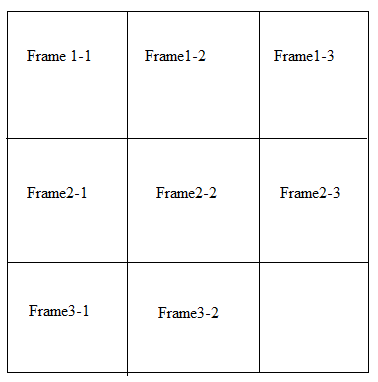
\includegraphics[scale = 0.4]{Images/Fig5}
    \caption{Convention for representing the frames in a 3x3 problem}
  \label{fig5}
\end{figure}


\subsection*{2x2 Problem}
\subsubsection*{Step 1: Identifying the similitude transformations}
As per Kunda, McGreggor and Goel \cite{paper}, I have defined the following similitude transformations which can possibly exist between two given frames of the problem:
\begin{enumerate}
\item Identity
\item Reflection (w.r.t a vertical axis)
\item Flip (w.r.t a horizontal axis)
\item Rotation by $90\,^{\circ}$
\item Rotation by $180\,^{\circ}$
\item Rotation by $270\,^{\circ}$
\item Ratio between the number of shapes (on a pixel level!)
\item Addition/ removal of shapes (difference in the number of shapes) (again on the level of pixels)
\end{enumerate}

Based on the frames in the reference matrix, it is first established if Frame1-2 is related to Frame1-1 by any of the first 6 transformations. If that is the case, then an estimated answer is directly generated by performing that transformation on Frame2-1. Otherwise, two estimate frames are created, where the number of shapes in the first estimate is, 
\\ \centerline{$NumberOfShapes(Frame2-1)$ * $NumberOfShapes(Frame1-2)$/ $NumberOfShapes(Frame1-1)$}
\\and the second one having, 
\\ \centerline{$|NumberOfShapes(Frame1-1)$ - $NumberOfShapes(Frame1-2)|$}
\\ The answer choice which is closest to this estimate is chosen as the correct answer.


To perform the visual comparison, each image corresponding to a frame is read from file and is stored as its associated RGB matrix. This is a square matrix (79x79) where the value of each element is equal to the RGB value of the corresponding pixel in the image. That is,\\
	\centerline{RGB Matrix A = $[a_{i,j}]$, where}\\
	\centerline{$[a_{i,j}]$ = RGBValue of $Pixel_{i,j}$ }\\
Since the image is black-and-white, the value of each element is either 0(black) or 255(white).

\subsubsection*{Step 2: Getting the estimate}
Let the RGB matrix of the Frame$i$-$j$ be represented as Fij. That is, the RGB matrix for Frame1-1 is F11, for Frame1-2 is F12 and for Frame2-1 is F21. Obtain the self-correlation value of F12 as a basis of comparison (to be explained soon). In general the process of computing the cross-correlation value of two matrices(m1 and m2) are found as follows\footnote{As outlined in the SciPy documentation \cite{web}}
	\begin{itemize}
		\item Find the inner product of m1 with the convex combination matrix \cite{math} [299, 587, 114] to obtain the luminance value for each pixel.
		\item We perform the above step so that when divided by a constant (in my case 1000.0), the elements in the resulting matrix are normalized and lie in the range [0,1].
		\item Repeat the above steps for m2 as well. Now we have two resultant matrices, say M1 and M2.
		\item Apply the \emph{SciPy} function \cite{web} \emph{correlate2d}, with the parameters being M1 and M2, to obtain an array of floating point numbers, which represent various measures of corelation between the two matrices.
		\item The maximum value among the array is the corelation measure of M1 with M2 (and in turn m1 with m2).
	\end{itemize}
So to obtain the self-corelation of F12, replace both m1 and m2 in the procedure listed above with F12. Call this value as $selfCorelation$.

Apply the first 6 transformations on F11 one-by-one and obtain a transformation matrix. So, we have
\begin{enumerate}
	\item For the identity transformation, the transformation matrix is same as F11.
	\item For reflection, obtain the transformed matrix using the \emph{PIL} utility \emph{transpose} \cite{pil} as,\\
		\hspace*{3cm}F11.transpose(FLIP\_LEFT\_RIGHT)
	\item For flip, similarly obtain the transformation matrix using the \emph{PIL} utility \emph{transpose} \cite{pil} as,\\
		\hspace*{3cm}F11.transpose(FLIP\_TOP\_BOTTOM)
	\item Obtain the transformation matrix for rotation by $90\,^{\circ}$, using the \emph{PIL} utility \emph{rotate} \cite{pil} as,\\
		\hspace*{3cm}F11.rotate(90)
	\item Obtain the transformation matrix for rotation by $180\,^{\circ}$, using the \emph{PIL} utility \emph{rotate} \cite{pil} as,\\
		\hspace*{3cm}F11.rotate(180)
	\item Obtain the transformation matrix for rotation by $270\,^{\circ}$, using the \emph{PIL} utility \emph{rotate} \cite{pil} as,\\
		\hspace*{3cm}F11.rotate(270)		
\end{enumerate}
Find the cross-correlation of the transformation matrix for each of the above 6 cases with F12. Check for an exact match between $selfCorelation$ and the above obtained cross-correlation (using the threshold described in Point 1 of Assumption 5). The one which falls within the permissible limits is the ``target'' transformation.

To obtain the estimate, perform this ``target'' transform on F21. Let the RGB matrix for the estimate be F\_estimate. This I define to be a ``strong'' estimate.

However if none of the 6 transformations give rise to a ``strong'' estimate, then two ``good enough'' estimates are created as described earlier. These estimates will have information about the number of shapes which needs to be there in the expected answer.

\subsubsection*{Step 3: Getting the answer from the answer choices}
Now we will either have a ``strong'' estimate or two ``good enough'' estimates. If the estimate is strong, then obtain the cross-correlation of the RGB matrix of each of the answer choices with F\_estimate. Check for an exact match (again using the threshold described in Point 1 of Assumption 5) for each of the answer choice with F\_estimate. The choice which gives the best match is the answer.

If the estimate is not strong, then we will try to find an answer with the ``good enough'' estimates, one at a time. First, choose the estimate which was selected based on the ratio transformation, and call it F\_weak. Scan through each of the answer choices, getting the cross-correlation value of their RGB matrix with F\_weak. If there is only 1 answer choice which falls within the threshold for exact match as described in point 3 of assumption 5, then declare that as the answer. If there is more than 1 choice (or no answer choice), then use the estimate based on the difference transformation. Find the cross-correlation of each of the answer choices with the RGB value of this weak estimate. Among the answer choices which fall withing the equivalence threshold described in point 2 of assumption 5, find the one closest to F\_weak. Declare that as the correct answer.

\subsection*{3x3 Problem}
\subsubsection*{Step 1: Generating estimates}
In the case of 3x3 problems, all estimates generated will be ``weak''. Three estimates are selected based on the frames in the reference matrix as follows,
\begin{enumerate}
	\item Ratio between the reference frames. Find the ratio of the number of shapes (by using the pixel information in the RGB matrix) of Frame1-3 and Frame1-2. Store this transformation matrix as F\_ratio.
	\item Difference between the reference frames. Find the difference between the number of shapes of Frame1-3 and Frame 1-2. Store this transformation matrix as F\_difference.
	\item Pairwise difference between the frames. Obtain the difference in the number of shapes between Frame1-3 and Frame1-2; between Frame1-2 and Frame1-2 and between Frame1-3 and Frame1-1. Compose these three into a transformation matrix as F\_pairwise.
\end{enumerate}

\subsubsection*{Step 2: Getting the correct answer choice}
Scan through the answer choices, and perform the following:
\begin{enumerate}
	\item Obtain the RGB matrix for the choice. Find the ratio of the number of shapes in Frame3-2 to the number of shapes in the answer choice. Perform the cross-correlation of this transformation with F\_ratio. If it is within the permissible threshold for ratio match add it to the list of potential answer choices.
	\item If the number of potential answer choices is just 1, then declare that as the correct answer.
	\item Else if that number is 0 (or greater than 1), find the difference in the number of shapes of Frame3-2 to that in the answer choices. Perform the cross-correlation of this transformation with F\_difference. If it is within the permissible threshold for difference match add it to the list of now potential answer choices.
	\item Again if this list has just one answer choice, then declare that as the correct answer.
	\item Else, find the pairwise difference of the each of the answer choices with the frames in row 3. That is, find the difference between the number of shapes in Frame3-2 and the answer choice; difference between the number of shapes in Frame3-2 and Frame3-1; and the difference between the number of shapes in Frame3-1 and the answer choice. Find the composite transformation matrix of this pairwise difference and perform the cross-correlation with F\_pairwise.
	\item Choose the answer choice which is closest to F\_pairwise and declare it as the correct answer.
\end{enumerate}

\subsection*{Propositional Solver}
The propositional solver does not vary with the dimensionality of the problem. It works similarly for both 2x2 as well as 3x3 problems. In this approach, a simple representation for each of the frames is extracted from the visual representation. There are 3 important representation files which are used to choose/eliminate the answer choices. They are as follows,
\begin{enumerate}
	\item \textit{Factor file}: This file indicates what are the structural transformations among the frames in the reference matrix.
	\item \textit{Base File}: This file assigns a base score for the ``target'' frame in the incomplete matrix. This assignment is based on the frames in the ``reference'' matrix, and is detailed in the next section.
	\item \textit{Target File}: This file contains the score for each of the answer choices. Based on this score, answer choices which are very far away from the base score will be eliminated.
\end{enumerate}

\subsubsection*{Step 1: Determining the factors}
This step has some overlap with Step 1 of the visual analogy solver. In this step, in addition to finding out which of the 8 transformations are in play, the shapes in common to the frames in the reference matrix will also be found out. 
\begin{enumerate}
	\item If the transformation is one among 1-6, then the common shape is the one in the reference frame.
	\item Else if the transformation is 7 or 8, then obtain the shape which needs to be in the answer by performing an intersection of the shapes in the reference frames.
	\item Write to the factor file, the transformation which is involved in the reference frames along with the shape(s) which are required to be present in the answer.
	\item These shapes are represented in a cannonical form, as shape0, shape1 and so on and not by its actual name.
\end{enumerate}

\subsubsection*{Step 2: Assigning a base score}
The base score is assigned based on the transformation established from the previous step.
\begin{enumerate}
	\item If the transformation is established as one of the affine transforms then the base score will be similar to the self-correlation of the reference frame.
	\item Else this score will be computed based on the composition of pixels in the frame. The score will determine the following characteristics of the frame,
		\begin{itemize}
			\item Number of shapes in the frame.
			\item Position/orientation of each of the shapes in the frame.
			\item Fill of the shape.
		\end{itemize}
	\item The score is in a particular range depending on each of the above 3 mentioned factors.
\end{enumerate}

\subsubsection*{Step 3: Choosing the correct answer}
\begin{enumerate}
\item Scan through each of the answer choices. If the transformation established in the previous steps is affine, then any answer choice which does not contain even one of the required shapes is eliminated. If at the end of this, there is only one choice in contention, declare that as the right answer.
\item Else, if there is more than one choice, (with the transformation being affine), then find the choice which has a score closest to the base score.
\item If the transformation is not affine, then perform the elimination as follows:
	\begin{itemize}
		\item Eliminate answer choices which do not have as many shapes as indicated in the factor file.
		\item Eliminate answer choices in which the number of shapes fall outside the indicated number of shapes based on the ratio transformation factor.
		\item If there is only one choice remaining then declare that as the answer.
	\end{itemize}
\item If there is more than one choice, again decide the answer based on which is closest to the reference score.
\end{enumerate}

\subsection*{Architecture of the Algorithm}
The overall visual solver's architecture is illustrated in Figure \ref{fig6} at a high level of abstraction. The 2x2 problem solver and the 3x3 problem solver are described in more detail in Figures \ref{fig7} and \ref{fig8}.

\begin{figure}[h!]
  \centering
    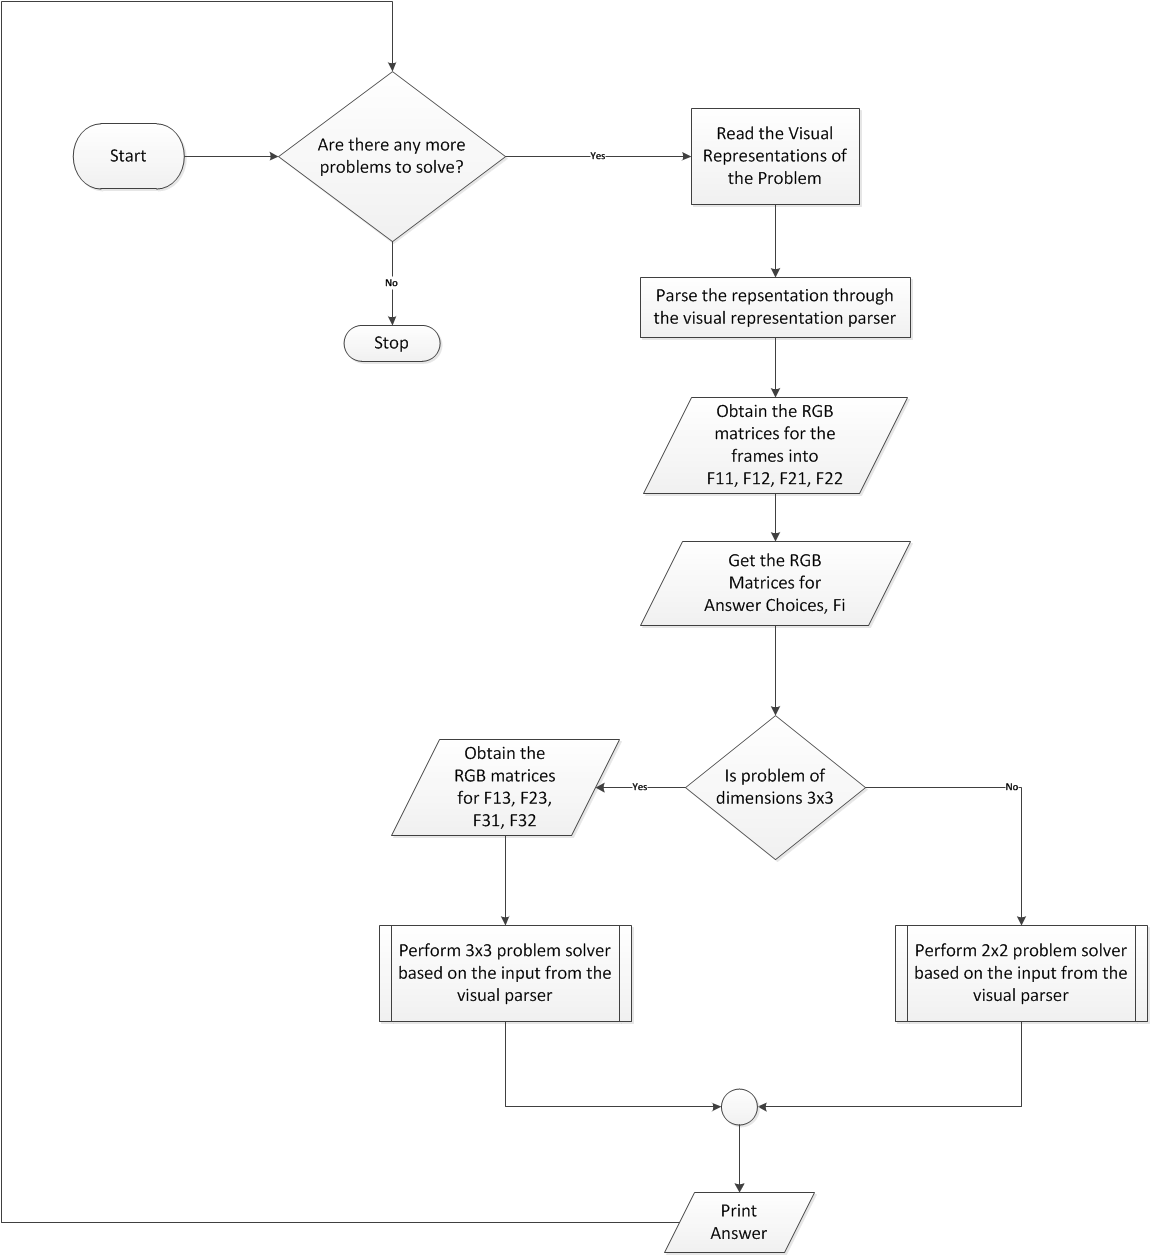
\includegraphics[scale = 0.35]{Images/Fig6}
    \caption{High-Level Architecture of the Visual Problem Solver}
  \label{fig6}
\end{figure}

\begin{figure}[h!]
  \centering
    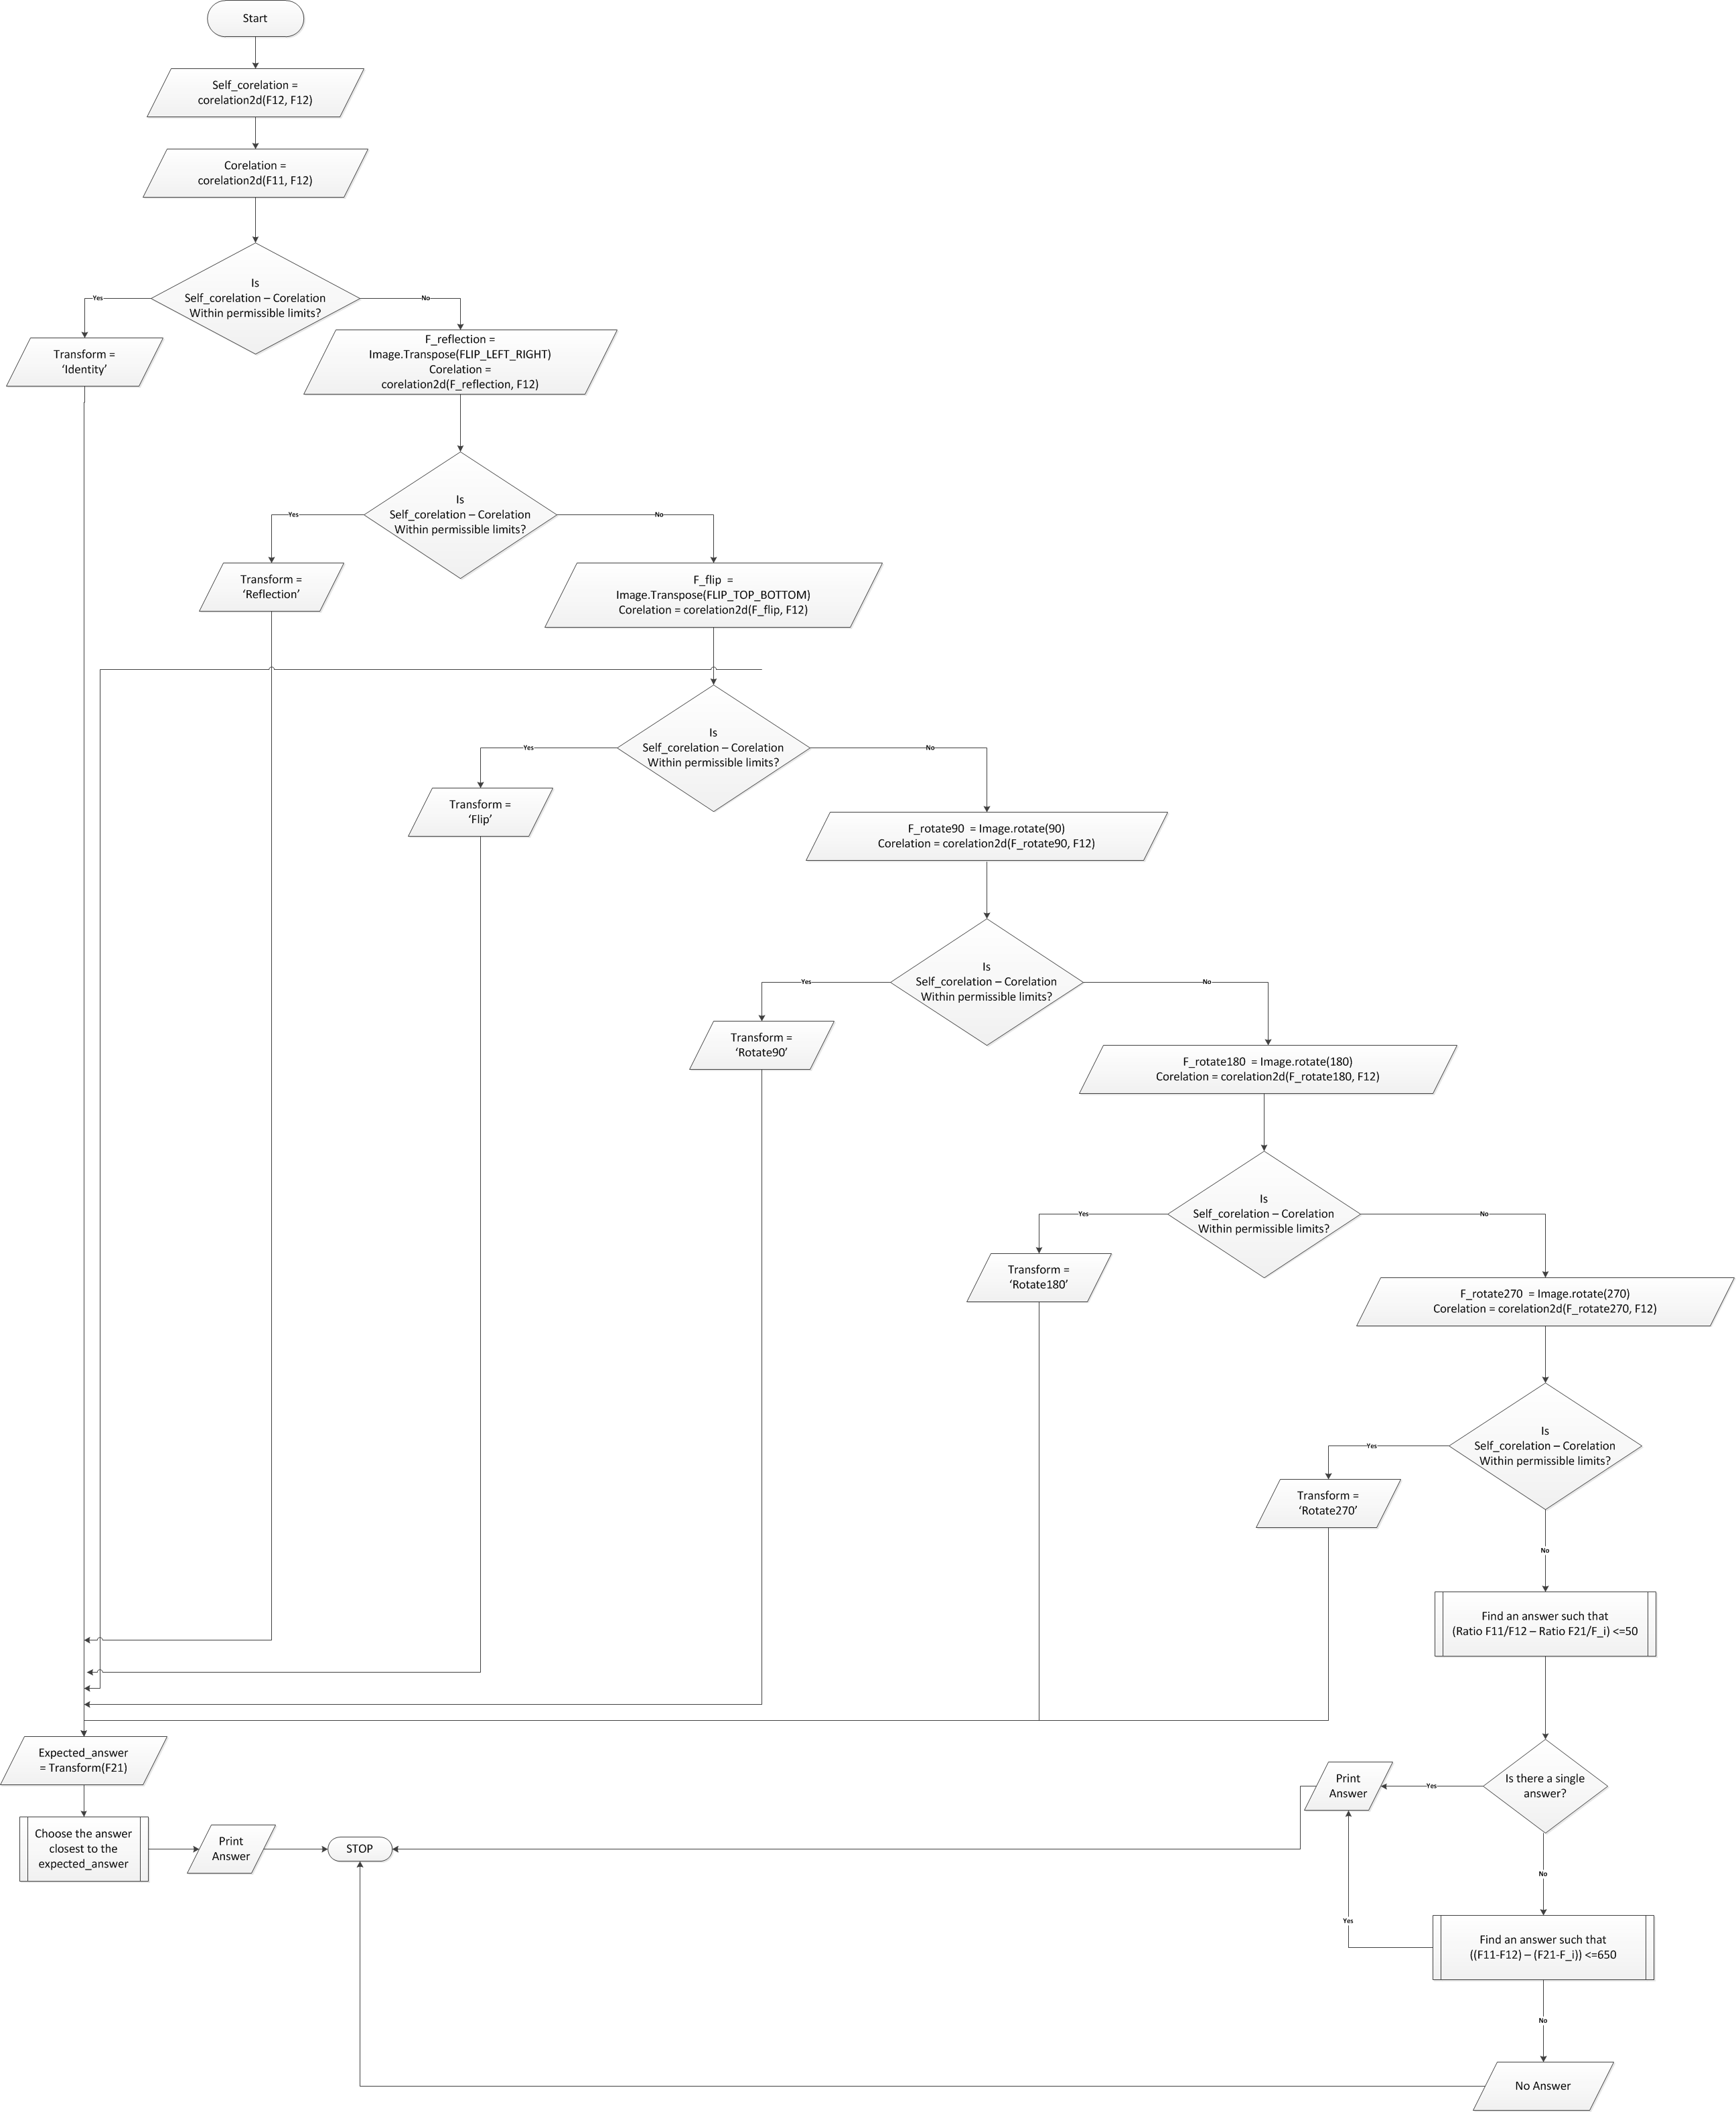
\includegraphics[scale = 0.25]{Images/Fig7}
    \caption{Architecture of the 2x2 Problem Solver}
  \label{fig7}
\end{figure}

\begin{figure}[h!]
  \centering
    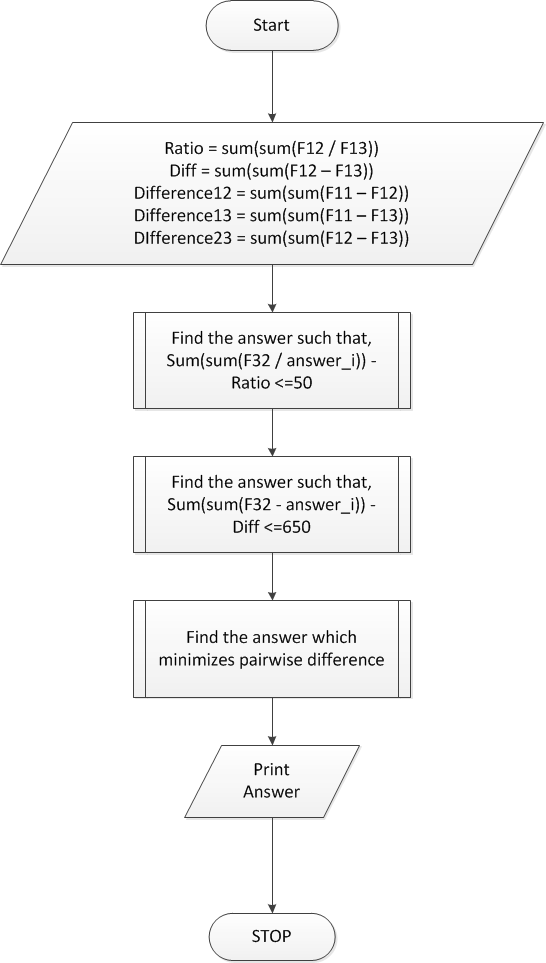
\includegraphics[scale = 0.35]{Images/Fig8}
    \caption{Architecture of the 3x3 Problem Solver}
  \label{fig8}
\end{figure}

The propositional solver's architecture is illustrated in Figure \ref{fig19} from a high-level of abstraction.
\begin{figure}[h!]
  \centering
    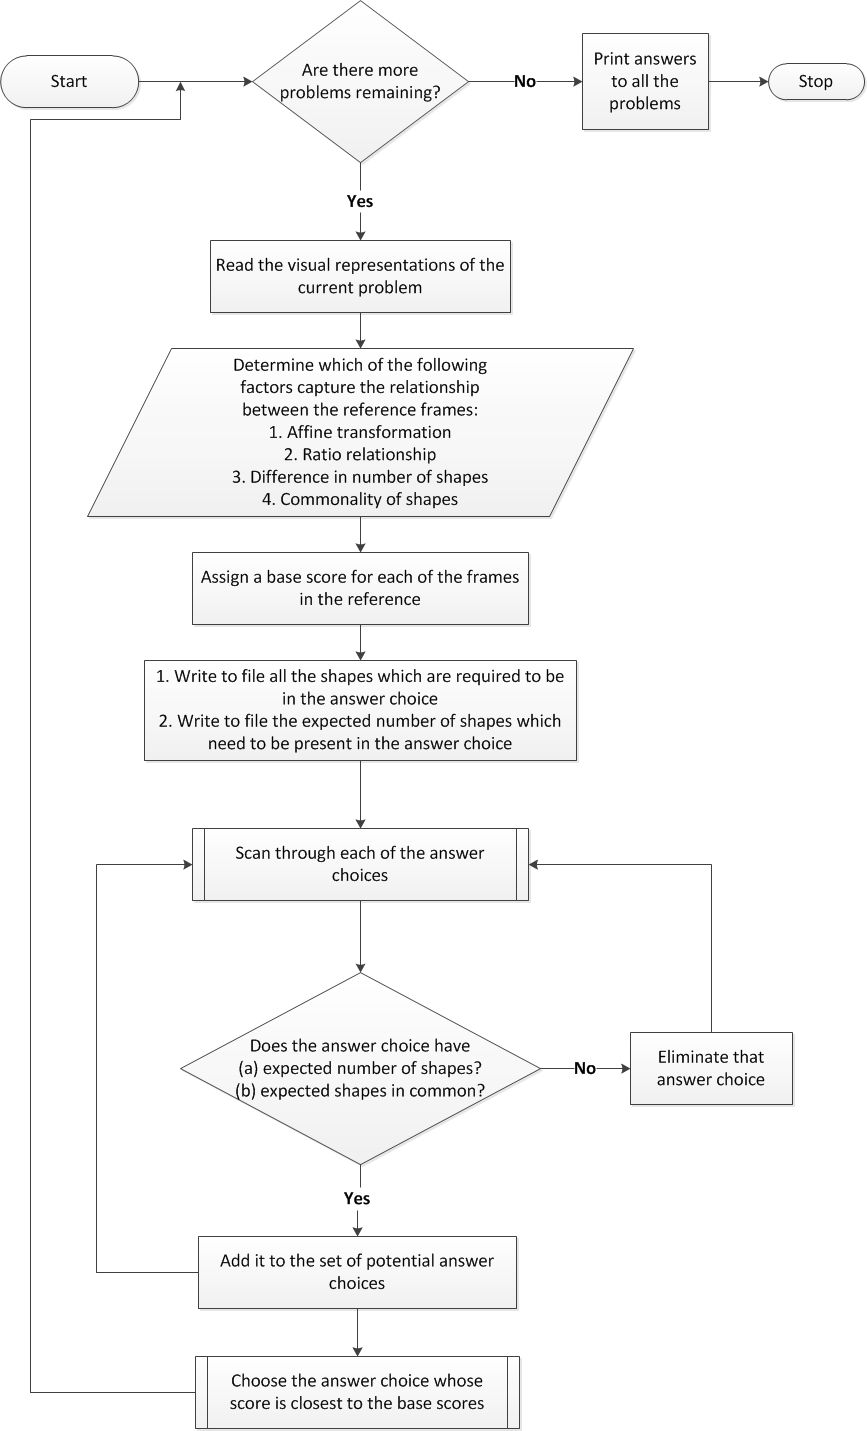
\includegraphics[scale = 0.35]{Images/fig9_flowchart}
    \caption{High-Level Architecture of the Propositional Problem Solver}
  \label{fig19}
\end{figure}

\subsection*{Tracing the algorithm for a problem}

Firstly the algorithm for the visual analogy solver is traced in the subsequent sub-sections. I have presented two instances of 2x2 problems and one of a 3x3 problem, which maximally traces through all the possibilities of the algorithm.
\subsubsection*{2x2 Problem - Example 1}
Figure \ref{fig9} represents a problem where one of the `traditional' transforms are used to determine the answer choice. The program proceeds as follows to find the answer,
\begin{figure}[h!]
  \centering
    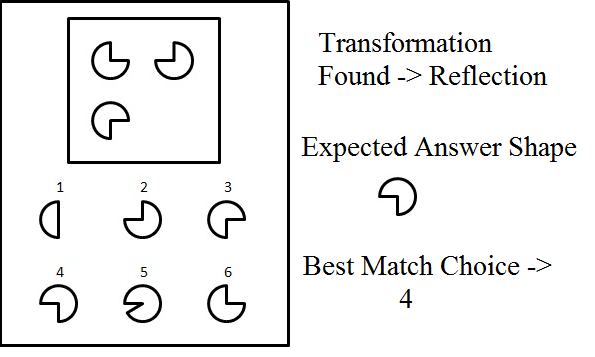
\includegraphics[scale = 0.5]{Images/Fig9}
    \caption{A sample 2x2 problem, with a `traditional' transformation}
  \label{fig9}
\end{figure}

\begin{enumerate}
	\item The 79x79 RGB matrix of frame1-1 and frame1-2 are stored as F11 and F12.
	\item The self-corelation value of F12 is found out to be 3844.0.
	\item For the identity transformation F11, the cross-corelation with F12 is found to be 1784.0.
	\item For the reflection transformation of F11, F\_Reflection, the cross-corelation with F12 is 3784.0. This is within the admissible threshold for equality and the transform is set to `REFLECT'.\\
	For the purpose of completeness the cross-corelation values for the other transforms are listed below,
	\begin{itemize}
		\item FLIP: 2881.0
		\item ROTATE90: 3691.0. \textbf{Note}: Although this transform also falls within the threshold, due to the fixed order in which the transforms are checked, reflection is given more priority over rotation.
		\item ROTATE180: 2901.0
		\item ROTATE270: 2004.0
	\end{itemize}
	\item Since the program has identified a `traditional' transformation, it does not bother with the non-traditional ones.
	\item Now the program formulates that the best expected answer should be a reflection of frame 2-1, which is also indicated in Figure \ref{fig9}.
	\item The self-corelation value for this image's RGB matrix (say F) is found to be 3884.0
	\item Each of the answer choices are represented by their RGB matrices and the cross-corelation with F is found out. They are listed out below,
		\begin{itemize}
			\item Choice 1: 2187.0
			\item Choice 2: 3458.0
			\item Choice 3: 4204.0
			\item Choice 4: 3803.0
			\item Choice 5: 4487.0
			\item Choice 6: 3689.0
		\end{itemize}
	\item Obviously the best match with the expected answer is choice 4, which turns out to be the right answer.
\end{enumerate}

\subsubsection*{2x2 Problem - Example 2}
In the example shown in Figure \ref{fig10}, none of the traditional transforms will give the right result. Again for the purpose of completeness, the significant comparison metrics for the 6 traditional transforms are given in the following list.

\begin{figure}[h!]
  \centering
    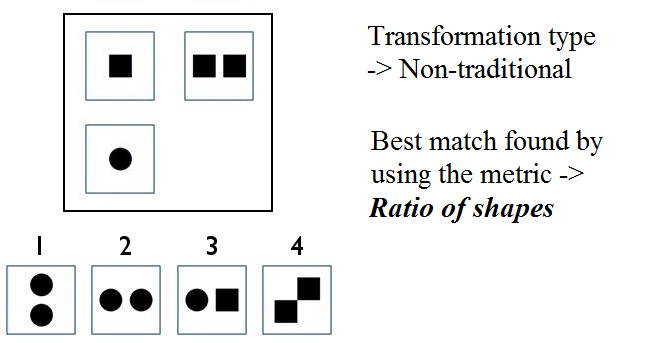
\includegraphics[scale = 0.5]{Images/Fig10}
    \caption{A sample 2x2 problem, with a `non-traditional' transformation}
  \label{fig10}
\end{figure}

\begin{enumerate}
	\item Self-corelation of frame1-2 : 1879.0
	\item Cross-corelation for IDENTITY : 2890.0
	\item REFLECTION : 2910.0
	\item ROTATE90 : 2453.0
	\item ROTATE180 : 2109.0
	\item ROTATE270 : 2907.0
\end{enumerate}

Obviously, none of the traditional transforms are even close to uncovering the true relation existing between frames1-1 and 1-2. Now the non-traditional transforms are applied.
\begin{itemize}
\item First the ratio between the shapes of frame1-1 and frame1-2 are found. The measure for this metric in this problem is found to be 729.0
\item The corresponding metric is computed for every pair involving frame2-1 and one of the answer choices. The values are as follows,
	\begin{enumerate}
		\item Ratio (Frame2-1, Choice 1): 604.0
		\item Ratio (Frame2-1, Choice 2): 731.0
		\item Ratio (Frame2-1, Choice 3): 575.0
		\item Ratio (Frame2-1, Choice 4): 834.0
	\end{enumerate}
\item From the listed values clearly choice 2 is the only choice within the threshold of 50. Hence it is declared as the result.\\
\textbf{Note}: Suppose the difference metric were applied to this problem instead of the ratio metric, the following values would have been obtained:
	\begin{enumerate}
		\item Diff(Frame1-1, Frame1-2): 1797.0
		\item Diff(Frame2-1, Choice 1): 907.0
		\item Diff(Frame2-1, Choice 2): 888.0
		\item Diff(Frame2-1, Choice 3): 1498.0
		\item Diff(Frame2-1, Choice 4): 1033.0
	\end{enumerate}
In such a scenario choice 3 would have been chosen as the right answer. It is just because I have given a higher priority to the ratio metric, choice 2 is chosen.\\
\textbf{Observation}: From the note it is clear that there can be two ways of viewing this problem. One is to say that with respect to the frame on the left, the number of shapes in the right frame has doubled (which is essentially what the ratio metric does). The second line of thought is to think that with respect to the left frame, a square has been added to the right frame (this is what the difference metric does). Hence depending on the line of thought, two possible solutions are possible, but it is purely out of personal taste that I have given more weight to the ratio metric than the difference metric (similar to the preference of reflection over rotation).
\end{itemize}
\subsubsection*{3x3 Problem - Example}
Compared to problems 4 and 6, problem 5, illustrated in Figure \ref{fig11} is tougher computationally. The trace of the algorithm through this problem will provide a sufficiently maximal example.

\begin{figure}[h!]
  \centering
    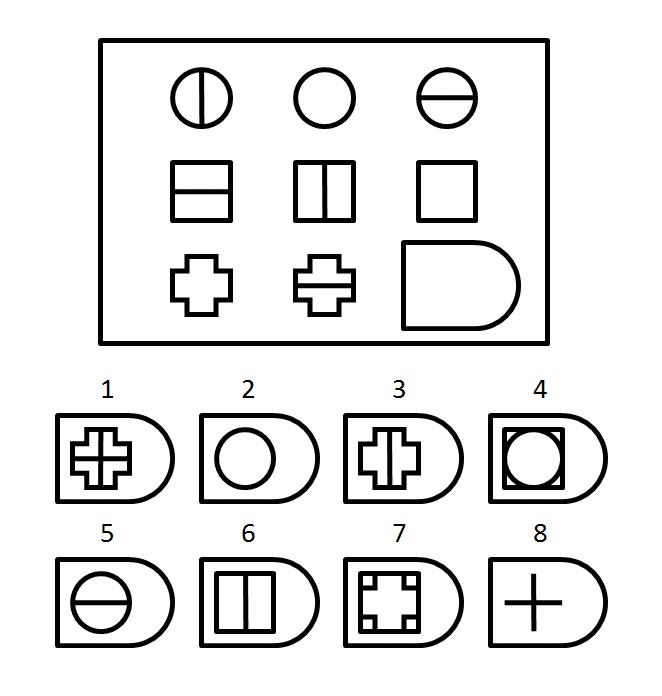
\includegraphics[scale = 0.25]{Images/Fig11}
    \caption{A computationally tough 3x3 problem}
  \label{fig11}
\end{figure}

\begin{enumerate}
\item The ratio metric is computed between frames1-2 \& 1-3 (451.0) and frames2-2 \& 2-3 (493.0). Since their difference is within the threshold, the ratio metric will be considered to filter out the answer choices.
\item The same is true of the difference metric too, since \\
	\hspace*{3cm}Diff frame1-2 - frame1-3 = 3451.0 and \\
	\hspace*{3cm}Diff frame2-2 - frame2-3 = 3309.0\\
	are within the threshold difference range (of 650.0).
\item The pairwise difference values are computed as follows, \\
	\hspace*{3cm}Diff frame1-1 - frame1-2 = 1931.0 and \\
	\hspace*{3cm}Diff frame1-2 - frame1-3 = 3451.0 and \\
	\hspace*{3cm}Diff frame1-1 - frame1-3 = 902.0
\item Applying the ratio metric for each pair of frame3-2 and the answer choices, we get the following values,
	\begin{enumerate}
		\item Ratio (frame3-2 / Choice 1): 509.0
		\item Ratio (frame3-2 / Choice 2): 149.0
		\item Ratio (frame3-2 / Choice 3): 464.0
		\item Ratio (frame3-2 / Choice 4): 613.0
		\item Ratio (frame3-2 / Choice 5): 198.0
		\item Ratio (frame3-2 / Choice 6): 704.0
		\item Ratio (frame3-2 / Choice 7): 402.0
		\item Ratio (frame3-2 / Choice 8): 453.0
		\end{enumerate}
\item From the above obtained values, choices 2, 4, 5, 6 are eliminated as they lie outside the defined threshold of 50 (from either 451.0 or 493.0)
\item Now for the remaining choices (1,3,7,8) the difference metric is applied, with the following results
	\begin{enumerate}
		\item Diff (frame3-2 - Choice 1): 4193.0
		\item Diff (frame3-2 - Choice 3): 3003.0
		\item Diff (frame3-2 - Choice 7): 4945.0
		\item Diff (frame3-2 - Choice 8): 3987.0		
	\end{enumerate}
\item In the above list, choices 1 and 7 fall outside the threshold range of 650.0 (from 3451.0 as well as 3309.0) and are subsequently eliminated.
\item The pairwise difference values are computed for the remaining choices (3 and 8) and the results are as follows
	\begin{enumerate}
		\item Diff (frame3-1 - frame3-2): 1731.0 (same for both answer choices obviously)
		\item Diff (frame3-1 - Choice 3): 1210.0
		\item Diff (frame3-2 - Choice 3): 3003.0
		\item Diff (frame3-1 - Choice 8): 2890.0
		\item Diff (frame3-2 - Choice 8): 3987.0 
	\end{enumerate}
\item The $ReferenceSum$ = 1931.0 + 3451.0 + 902.0 = 6284.0
\item The $ChoiceSum$ for Choice 3 = 1731.0 + 1210.0 + 3003.0 = 5944.0
\item The $ChoiceSum$ for Choice 8 = 1731.0 + 2890.0 + 3987.0 = 8608.0
\item Obviously the difference between $ChoiceSum$ and $ReferenceSum$ is least for choice 3, which is declared as the right answer.
\end{enumerate}

The following sub-section provides an example of the propositional problem solver. Since it works in the same way for 2x2 as well as 3x3 problems, I am using a ``hard'' 3x3 problem to trace through the algorithm.

\subsubsection*{3x3 Problem - Propositional Problem Solver}
The example illustrated in Figure \ref{fig12} is used to trace the propositional problem solver.

\begin{figure}[h!]
  \centering
    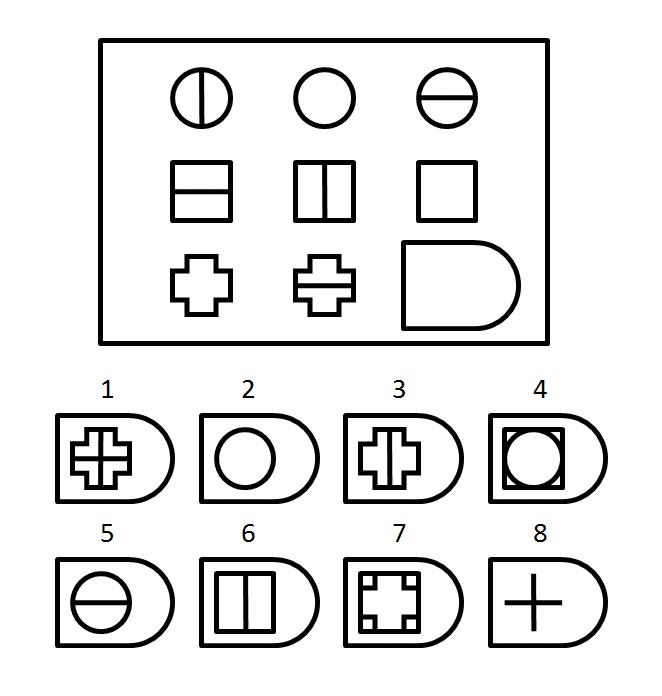
\includegraphics[scale = 0.25]{Images/Fig11}
    \caption{Illustrative 3x3 problem for Propositional Solver}
  \label{fig12}
\end{figure}

The steps of the algorithm are as follows:
\begin{enumerate}
\item Going through the first row, the algorithm finds that there is no affine transformation possible.
\item It finds out from the first and second rows that the total number of shapes in each row is a constant.
\item From the first row the program finds out that the common shape is the outer shape, or shape0 (which corresponds to the circle in this case). So the answer choice must have shape0 of row 3, which is the outer cross symbol.
\item The factor file is created, with the factors written as,
	\begin{itemize}
		\item Ratio of shapes
		\item Difference in shapes
		\item Pairwise difference of shapes
		\item Expected number of shapes based on the above 3 factors = 2
	\end{itemize}
\item The base score is computed for the Frame3-2 using a correlation measure as 18+288+297 = 603.
\item Each of the answer choices are scanned, and the following results are obtained:
	\begin{itemize}
		\item Choice 1: Number of shapes: 3 == Eliminated
		\item Choice 2: Number of shapes: 1 == Eliminated
		\item Choice 3: Number of shapes: 2 
						Is shape0 present in this choice: Yes == Added to potential answer choices
		\item Choice 4: Number of shapes: 2
						Is shape0 present in this choice: No == Eliminated
		\item Choice 5: Number of shapes: 2
						Is shape0 present in this choice: No == Eliminated
		\item Choice 6: Number of shapes: 2
						Is shape0 present in this choice: No == Eliminated
		\item Choice 7: Number of shapes: 2
						Is shape0 present in this choice: Yes == Added to potential answer choices
		\item Choice 8: Number of shapes: 2
						Is shape0 present in this choice: No == Eliminated
	\end{itemize}
\item Compute the correlation score of the potential answer choices.
	\begin{itemize}
		\item Score of Choice 3: 20+312+347 = 679
		\item Score of Choice 7: 113+89+16 = 218
	\end{itemize}
\item The choice closest to the base score is Choice 3, which is then selected as the answer.
\end{enumerate}

\section{Implementation and Execution Details}

The entire project is implemented in Python, with the basic image processing tasks handled by Python's Imaging Library (PIL) and the numeric manipulations of the images being performed through SciPy and NumPy. The following are some of the important functions utilized in these libraries,
\begin{enumerate}
	\item Image.transpose - with the parameter FLIP\_LEFT\_RIGHT it performs reflection and with the parameter FLIP\_TOP\_BOTTOM it performs a flip
	\item Image.rotate - rotates the image by the angle given as the parameter
	\item Image.open() - open the image given in the parameter as a PIL object
	\item numpy.asarray() - takes a PIL object and constructs its RGB matrix.
	\item scipy.corelation2d() - takes two matrices as input and returns their corelation vector/array
	\item os.listdir() - lists the contents of the path given as a parameter
\end{enumerate}
To run the project, execute the command, \\
	\hspace*{3cm} python Arvind\_Krishnaa\_Jagannathan\_Project\_4.py \\ \\
The project has the following dependencies
\begin{enumerate}
\item \textbf{SciPy}	\url{http://sourceforge.net/projects/scipy/files/scipy/0.11.0/}
\item \textbf{NumPy}	\url{http://sourceforge.net/projects/numpy/files/NumPy/1.7.0b2/}
\item \textbf{PIL (Python Imaging Library)}	\url{http://effbot.org/downloads/\#pil}
\end{enumerate}
Also python-2.7 is the preferred interpreter.

When run, the program will perform the visual solver algorithm first, followed by the propositional solver. The answers to problems 1-10 will be printed at the end, in the summary section for both the methods. For problems 11 and 12, the answer will be printed as ``None'' for both the cases. Once the problems are available, the empty folders 11 and 12 in the directory ``Representations'' needs to be replaced with the folders submitted along with this report. Correspondingly, the folders 11 and 12 in the ``Generated\_Propositional\_Representations'' will be automatically written with the requried propositions for problems 11 and 12.

\section{Introspection}
\subsection*{Time Complexity}
\subsubsection*{For the visual problem solver}
Since all operations involve pixel-by-pixel comparison, assuming on average an image being of dimensions nxn, then the time complexity will be atleast \bigO{($n^2$)}. However, in addition to simple pixel comparison, the program needs to determine the number of shapes (or pixels) newly added, deleted or modified between two frames. If these are represented by N, M and K respectively, then this process itself will have a time complexity of \bigO{($N! * M! * K!$)}. Since these two are independent processes, the overall time complexity for the problem will be \\
\hspace*{3cm}\bigO{($n^2$ * $N!$ * $M!$ * $K!$)}
\subsubsection*{For the propositional problem solver}
The propositional problem solver is a 2-step process. The first step is to generate the propositions for the problem. Assuming there are a total of N1, N2 (and N3 in case of a 3x3 problem) shapes in a row of the problem. Obviously the time taken to find the common shape among them will be \bigO{(max($N1$, $N2$, $N3$))}. Also the time taken for determining the correlation score depends on the dimensionality of the problem, and is atleast \bigO{($n^2$)} for nxn problem. In addition, since the correlation measure is derived in a manner similar to the visual solver, there is an additional overhead of \bigO{($N1! * N2! * N3!$)}. Thus the overall time complexity will be \\
\hspace*{3cm}\bigO{($n^2$ * $N1!$ * $N2!$ * $N3!$ * max($N1$, $N2$, $N3$))}

\subsection*{Space Complexity}
\subsubsection*{For the visual problem solver}
Assuming that each frame of the problem is represented as a nxn image. Then the space required for one frame is \bigO{($n^2$)}. Now let M be the total number of frames of the problem (including the reference frames and answer choices). Then the overall space complexity will be \\
\hspace*{3cm}\bigO{($n^2$ * $M$)}
\subsubsection*{For the propositional problem solver}
The propositional problem solver, utilizes the visual representations as well. Thus its space complexity will be = Space Complexity of Visual Problem Solver + Space Complexity for storing the extracted representations. \\
If there are K answer choices then there will be a representation for each of the answer choices. In addition there are 2 more representation files, the factor file and the base score file. Thus the space complexity for storing the representations becomes, \bigO{($K$+3)} = \bigO{($K$)}. Thus the overall space complexity becomes \\
\hspace*{3cm}\bigO{(($n^2$ * $M$) + $K$)}

\subsection*{Fixing the threshold limits}
Obviously when dealing with a lossy image format like JPG (which is used to store each individual frame), even if two images appear exactly alike, they will most certainly fail a test conducted by simply matching individual pixels. To slightly improve the chances of two alike images being reported as alike, I have chosen to instead compare them based on the corelation measure of the pixel matrix instead of the individual pixels themselves. Even then, due to the presence of noise, the value of the corelation will also not be exactly the same. I have performed empirical tests, based on the problems given as part of this project to derive the threshold values described in my assumptions. There is no solid scientific backing behind the values and some future example may prove that these thresholds are too restrictive or lenient. The correctness of the threshold may vary with the problem as well as the approach being used (visual vs. propositional).

\subsection*{Implicit Priority}
In case of either 2x2 or 3x3 problems, the order in which the metrics are checked, will impose an implicit prioritization of one metric over the other. For instance, as indicated earlier, the `target' transform for problem 1, is identified as `REFLECTION' instead of `ROTATE90', because the REFLECTION transformation is checked first (ahead of ROTATE90). Similarly for problem 2, the program deduces that the relation is to multiply the existing shape (as opposed to adding a square), because the ratio metric is checked before the difference metric. 

Such a prioritization exists even in the propositional approach. Mirroring the visual approach, REFLECTION will be given priority over ROTATION and RATIO metric will be given priority over ROTATION. The establishing of priorities can be seen in the order in which factors are listed in the factor file.

\subsection*{Experimental Analysis}
The two approaches of the analogy solver were tested against a fairly tough 3x3 problems. The first problem is shown in Figure \ref{exp1}. By splitting up this problem into the individual frames, the visual solver was able to produce the correct answer as 7 (which is right). 
\begin{figure}[h!]
  \centering
    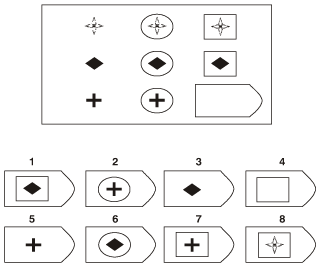
\includegraphics[scale = 0.45]{Images/Exp1}
    \caption{Experimental Problem}
  \label{exp1}
\end{figure}

For the propositional approach, the answer was derived based on a series of eliminations. The sequence of eliminations were,
\begin{enumerate}
	\item Choice 1,3,4,6,8 were eliminated since the required shape was not present..
	\item Choice 5 is eliminated as it does not have the required \textit{number} of shapes.
	\item Between choices 2 and 7, the correlation score of 7 was closest to the base score and is declared as the answer.
\end{enumerate}

\subsection*{Ablation Experiment}
The toughest experimental problem presented to the program is illustrated in Figure \ref{exp2}. The obvious difficulty with this problem is to be able to extract each of the individual frames without loss of information near the boundaries. Also once extracted, it was found that the program gave a completely wrong answer (E as opposed to B for the visual method and D as opposed to B for the propositional method). On further inspection, it was observed that there was significantly high levels of noise in each of the answer choice frames. After spending some significant time removing this noise, the program was run again; this time giving the right answer in both cases. This clearly indicates that the entire success or failure of both the algorithms depends on the quality of the input image.

\begin{figure}[h!]
  \centering
    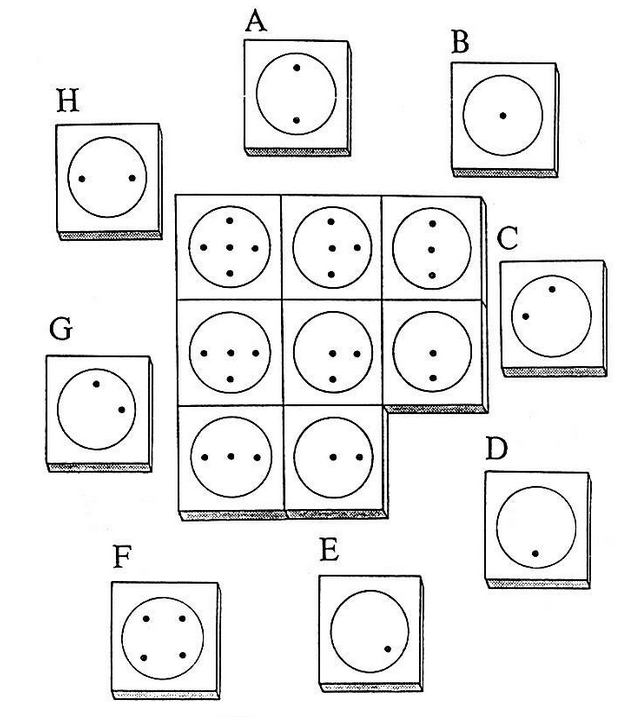
\includegraphics[scale = 0.25]{Images/Exp2}
    \caption{Ablation Experiment}
  \label{exp2}
\end{figure}

\section{Comparative analysis of the Visual and the Propositional Solver}
I will be comparing the two approaches on the following parameters,
\begin{itemize}
	\item Efficiency of the algorithm
	\item Accuracy of the algorithm
	\item Generalizability of the algorithm
	\item Limits of the algorithm
\end{itemize}

\textbf{Note}: Obviously the two possible ``generic'' approaches to solving a multiple choice problems are reflected in this project. In the purely visual solver approach, an answer is generated only from the facts available in the question (the ``forward'' approach). The propositional method however, reflects the ``process of elimination'' approach. Every answer choice is examined and the one which most seems to be a ``best fit'' is selected as the solution (the ``backward'' approach). These can be mapped to the approaches discussed in the class lecture.

\subsection*{Efficiency of the algorithm}
As discussed earlier, both the time complexity and the space complexity of the propositional solver are higher than that of the visual solver. This is because the propositional solver ``piggybacks'' on the data from the visual solver and has the additional overhead of creating propositions and processing them. However, had I tried to derive the propositions from the image in the same syntax as the one I had used for project 2, the performance would have further deteriorated as in addition to pixel processing, it would be necessary to group these pixels into shapes and the shapes into frames.

\subsection*{Accuracy of the algorithm}
In the 10 given problems, both the visual and the propositional solvers gave the same (correct) results. In general, from the two experimental problems although there is no obvious difference in the accuracy of the two approaches, I am inclined to conclude that the visual method may be more accurate in harder, or other unseen problems. This is because the process of finding the common shape among frames may fail in certain cases. For some problems, this may not even be a criteria in selecting the correct answer.

\subsection*{Generalizability of the algorithm}
Both the algorithms are very generalizable within the realms of 2x2 and 3x3 problems. However they may not be necessarily scalable. The time taken for each of the approaches to generate a solution is directly proportional to the size of the image. For instance if the input images are of dimensions 100x100, then the time taken to produce a solution will almost double. 

Also, in these approaches, the influence of the second row is not taken into consideration at all. It assumes that the third row mirrors the structure of the first row. So for problems where the transformation of the third row either depends only on the second row, or on a composition of the transformations of the first and second row, these two approaches may not work out.

The propositional method can be extended beyond 3x3 problems as well, whereas the visual method (in its current implementation) cannot. However, for the propositional method to work well, a lot of computation is required, especially for finding the shape in common. The answer for these higher dimension problems generated by the proposition method may or may not be correct. However, the visual method will not even produce an answer.

\subsection*{Limits of the algorithm}
\begin{enumerate}
\item As mentioned previously, the visual method cannot solve problems other than 2x2 and 3x3. However, both these methods are unable to uncover subtle relationships among frames in problems such as the one in Figure \ref{con1}.

\begin{figure}[h!]
  \centering
    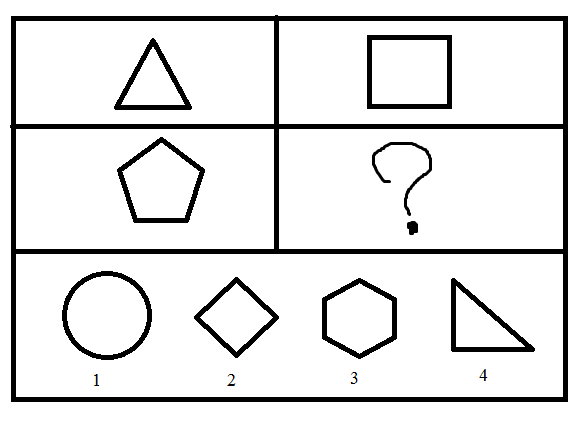
\includegraphics[scale = 0.3]{Images/con1}
    \caption{A subtle relationship that is not uncovered}
  \label{con1}
\end{figure}

\item Both the methods require the input images to be noise-free. However since the propositional method works by grouping clusters of pixels, it is slightly more tolerant to image noise than the visual method.
\end{enumerate}

\begin{thebibliography}{10}
\bibitem{paper} Kunda, Maithilee, Keith McGreggor, and Ashok Goel. "Taking a look (literally!) at the Raven’s intelligence test: Two visual solution strategies." Proc. 32nd Annual Meeting of the Cognitive Science Society, Portland. 2010.

\bibitem{math} Image Compression in JPEG Standard. Retrieved from \url{http://www.whydomath.org/node/wavlets/imagebasics.html}

\bibitem{web} SciPy and NumPy online documentation. Retrieved from \url{http://docs.scipy.org/doc/}

\bibitem{pil} Python Imaging Library. Retrieved from \url{http://www.pythonware.com/products/pil/}

\end{thebibliography}
\end{document}
